\subsection*{Одноканальная СМО}
\addcontentsline{toc}{subsection}{Одноканальная СМО}

\textbf{Задание:}\\
Реализовать одноканальную СМО на языке программирования Python.\\

\textbf{Решение:}\\
\textit{СМО с бесконечной очередью} -- это СМО, в которой всегда есть места в очереди и если требование приходит, в момент, когда обслуживающее устройство занято, то оно не получает немедленного отказа, а может стать в очередь и ожидать освобождения обслуживающего устройства.\\

На вход одноканальной СМО с бесконечной очередью поступает пуассоновский поток требований с интенсивностью $\lambda$.\\
Интенсивность пуассоновского потока обслуживания -- $\mu$.\\
Дисциплина очереди естественная: кто раньше пришёл, тот раньше и обслуживается.\\
Число мест в очереди не ограничено.

\subsubsection*{Реализация модели}
Данная модель была реализована на языке программирования Python. Для начала был создан класс \textit{QueuingSystemWithInfinityQueue}, в котором реализованы все необходимые методы.\\

Данная функция принимает на вход параметр $\lambda$, параметр $\mu$ и время моделирования системы в условных единицах. (Рисунок \ref{fig:queuing_system_with_infinity_queue_params})
\begin{figure}[h]
	\centering 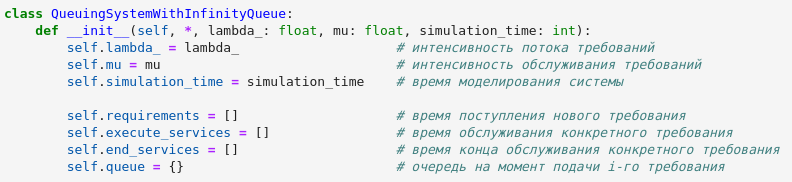
\includegraphics[scale=0.62]{queuing_system_with_infinity_queue_params}
	\caption{Параметры модели}
	\label{fig:queuing_system_with_infinity_queue_params}
\end{figure}

\newpage
Был реализован метод \textit{generate\textup{\_}requirements}, который генерирует поток требований в соответствии с пуассоновским законом распределения. (Рисунок \ref{fig:queuing_system_with_infinity_queue_generate_requirements})
\begin{figure}[h]
	\centering 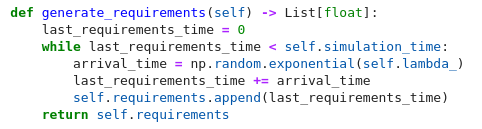
\includegraphics[scale=0.62]{queuing_system_with_infinity_queue_generate_requirements}
	\caption{Реализация метода генерации требований}
	\label{fig:queuing_system_with_infinity_queue_generate_requirements}
\end{figure}

Был реализован метод \textit{get\textup{\_}service\textup{\_}times}, который в соответствии с пуассоновским законом задаёт каждому требованию его время обработки. (Рисунок \ref{fig:queuing_system_with_infinity_queue_get_service_times})
\begin{figure}[h]
	\centering 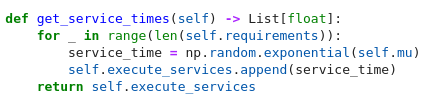
\includegraphics[scale=0.62]{queuing_system_with_infinity_queue_get_service_times}
	\caption{Реализация метода задания обработки требований}
	\label{fig:queuing_system_with_infinity_queue_get_service_times}
\end{figure}

Был реализован метод \textit{get\textup{\_}service\textup{\_}end}, который считает сколько времени провело требование в системе. (Рисунок \ref{fig:queuing_system_with_infinity_queue_get_service_end})
\begin{figure}[h]
	\centering 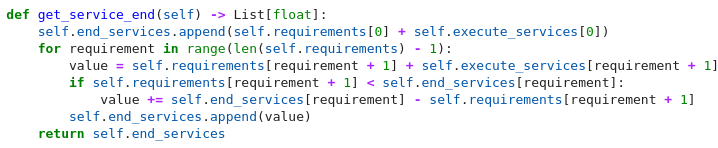
\includegraphics[scale=0.62]{queuing_system_with_infinity_queue_get_service_end}
	\caption{Реализация метода подсчёт времени требования в системе}
	\label{fig:queuing_system_with_infinity_queue_get_service_end}
\end{figure}

\newpage
Был реализован метод \textit{get\textup{\_}queue}, который для каждого требования сопоставляет количество требований, который находятся перед ним в очереди. (Рисунок \ref{fig:queuing_system_with_infinity_queue_get_queue})
\begin{figure}[h]
	\centering 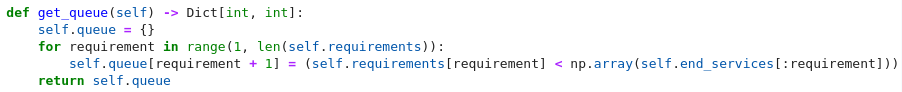
\includegraphics[scale=0.62]{queuing_system_with_infinity_queue_get_queue}
	\caption{Реализация метода нахождения количества требований в очереди перед текущим требованием}
	\label{fig:queuing_system_with_infinity_queue_get_queue}
\end{figure}

Был реализован метод \textit{get\textup{\_}features}, который рассчитывает основные характеристики модели. (Рисунок \ref{fig:queuing_system_with_infinity_queue_get_features})
\begin{figure}[h]
	\centering 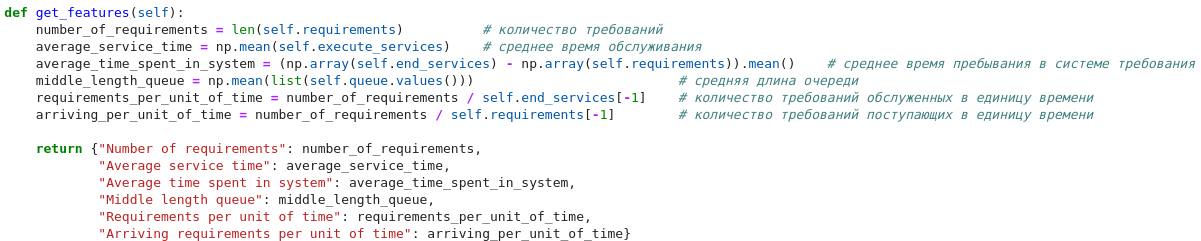
\includegraphics[scale=0.62]{queuing_system_with_infinity_queue_get_features}
	\caption{Реализация метода нахождения характеристик модели}
	\label{fig:queuing_system_with_infinity_queue_get_features}
\end{figure}

Характеристики модели:
\begin{enumerate}[topsep=0pt,itemsep=-1ex,partopsep=1ex,parsep=1ex]
	\item количество требований;
	\item среднее время обслуживания;
	\item среднее время пребывания в системе требования;
	\item средняя длина очереди;
	\item количество требований обслуженных в единицу времени;
	\item количество требований поступающих в единицу времени;
\end{enumerate}

\newpage
Если задать параметры модели: $\lambda = 1$, $\mu = 2$, \textit{simulation\textup{\_}time} = 100, то получаются следующие результаты. (Рисунок \ref{fig:queuing_system_with_infinity_queue_result})
\begin{figure}[h]
	\centering 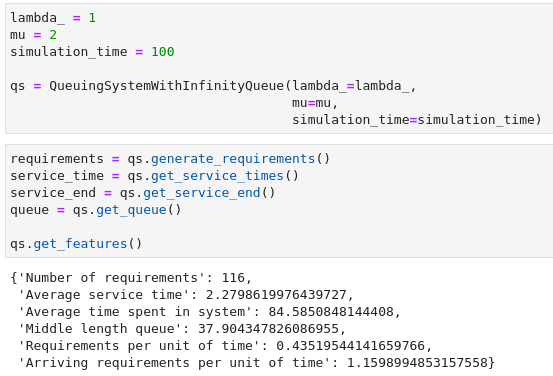
\includegraphics[scale=0.62]{queuing_system_with_infinity_queue_result}
	\caption{Результаты модели при $\lambda = 1$, $\mu = 2$, \textit{simulation\textup{\_}time} = 100}
	\label{fig:queuing_system_with_infinity_queue_result}
\end{figure}